
%(BEGIN_QUESTION)
% Copyright 2011, Tony R. Kuphaldt, released under the Creative Commons Attribution License (v 1.0)
% This means you may do almost anything with this work of mine, so long as you give me proper credit

Connect the necessary wires so that this temperature transmitter sends a 4-20 mA current signal to channel 1 of the analog input card on the PLC, assuming the temperature transmitter will be configured for a {\it 3-wire RTD} sensor:

$$\includegraphics[width=15.5cm]{i03430x01.eps}$$


\vskip 20pt \vbox{\hrule \hbox{\strut \vrule{} {\bf Suggestions for Socratic discussion} \vrule} \hrule}

\begin{itemize}
\item{} Students very commonly mis-interpret the symbols drawn next to the input terminals of an RTD transmitter, especially the terminals which must be made common to each other at the sensor.  One of the most popular misconceptions  is to think that those terminals shown common to each other by the symbol are already joined together {\it inside the transmitter}.  Explain why this interpretation cannot be true, based on how you know 3-wire and 4-wire RTD circuits are designed to work.
\item{} What type(s) of wire should be used to connect the RTD to the input terminals on the transmitter?  Should platinum wires be used (to match the RTD's wire type) or may regular copper wires be used?
\end{itemize}

\underbar{file i03430}
%(END_QUESTION)





%(BEGIN_ANSWER)


%(END_ANSWER)





%(BEGIN_NOTES)

Wiring solution:

$$\includegraphics[width=15.5cm]{i03430x02.eps}$$


%INDEX% Pictorial circuit review (analog signal wiring to PLC)

%(END_NOTES)


